\documentclass{report}
\usepackage[T1]{fontenc} % Fontes T1
\usepackage[utf8]{inputenc} % Input UTF8
\usepackage[backend=biber, style=ieee]{biblatex} % para usar bibliografia
\usepackage{csquotes}
\usepackage[portuguese]{babel} %Usar língua portuguesa
\usepackage{blindtext} % Gerar texto automaticamente
\usepackage[printonlyused]{acronym}
\usepackage{hyperref} % para autoref
\usepackage{graphicx}
\graphicspath{ {imagens/} }

\bibliography{bibliografia}


\begin{document}
%%
% Definições
%
\def\titulo{Sistemas operativos}
\def\data{06/12/2020}
\def\autores{Bruno Gomes, João Almeida}
\def\autorescontactos{(103320) brunofgomes@ua.pt, (103908) joao.artur@ua.pt}
\def\versao{VERSAO}
\def\departamento{Departamento de Eletrónica, Telecomunicações e Informática}
\def\empresa{Universidade de Aveiro}
\def\logotipo{ua.pdf}
%
%%%%%% CAPA %%%%%%
%
\renewcommand{\contentsname}{Índice}
\begin{titlepage}

\begin{center}
%
\vspace*{50mm}
%
{\Huge \titulo}\\ 
%
\vspace{10mm}
%
{\Large \empresa}\\
%
\vspace{10mm}
%
{\LARGE \autores}\\ 
%
\vspace{30mm}
%
\begin{figure}[h]
\center
\includegraphics{\logotipo}
\end{figure}
%
\vspace{30mm}
\end{center}
%
\begin{flushright}
\versao
\end{flushright}
\end{titlepage}

%%  Página de Título %%
\title{%
{\Huge\textbf{\titulo}}\\
{\Large \departamento\\ \empresa}
}
%
\author{%
    \autores \\
    \autorescontactos
}
%
\date{\data}
%
\maketitle

\pagenumbering{roman}

%%%%%% RESUMO %%%%%%
\begin{abstract}
O principal objetivo deste trabalho visa a mostrar os diferentes tipos de sistemas operativos que têm vindo a ser criados ao longo do tempo.

Vamos introduzir o conceito de 'sistema operativo', para dar um noção geral do 
que vai ser falado neste trabalho. Iremos falar do Windows, Linux, IOS e macOS. 

Basicamente vamos falar da história e evolução de cada um, e como têm
contribuído para a evolução do meio em que vivemos hoje. Adicionalmente, este trabalho pretende mostrar as diferentes funcionalidades e potencialidades menos evidentes que tenham passado despercebidas pelos utilizadores, de cada um dos sistemas operativos que irão ser falados.

Anexamente, este trabalho pretende evidenciar a inovação, e facilidade de acesso a um panóplia de conteúdos e ferramentas que têm vindo a facilitar a vida de praticamente toda a população mundial, e que de certa forma tem vindo a criar uma certa dependência, nas pessoas que os usam, devido ao facto de o sistema operativo ser um ferramenta poderosa, e essencial nos computadores dos dias de hoje.

Também iremos falar da utilização de 'virtual boxes', que são utilizadas para simular ambientes de trabalho de um sistema operativo escolhido pelo utilizador, dentro do sistema operativo originalmente instalado na sua máquina.

Para concluir este resumo, qualquer pessoa que esteja interessada em saber mais sobre sistemas operativos, pode consultar este trabalho, pois desta maneira ficará a ter uma ideia geral do assunto.
\end{abstract}

%%%%%% Agradecimentos %%%%%%
% Segundo glisc deveria aparecer após conclusão...
\renewcommand{\abstractname}{Agradecimentos}
\begin{abstract}
Eventuais agradecimentos.
Comentar bloco caso não existam agradecimentos a fazer.
\end{abstract}


\tableofcontents
% \listoftables     % descomentar se necessário
% \listoffigures    % descomentar se necessário


%%%%%%%%%%%%%%%%%%%%%%%%%%%%%%%
\clearpage
\pagenumbering{arabic}

%%%%%%%%%%%%%%%%%%%%%%%%%%%%%%%%
\chapter{Introdução}
\label{chap.introducao}

Para começar, podemos afirmar que maior parte da população sabe para que serve um sistema operativo, mas o que é um sistema operativo ao certo?

Basicamente, um sistema operativo consiste num conjunto de programas que permite criar uma interface entre o computador e o usuário do mesmo, ou seja permite gerir vários recursos do computador, tais como a memória, definição de processos que precisam de mais atenção do processador ou placa gráfica, o sistema operativo também permite ao usuário criar um sistema de arquivos para guardar qualquer tipo de documentos que o usuário queira, criando desta forma um ambiente de trabalho fácil de organizar e navegar. Resumindo e concluindo é o sistema operativo que permite a comunicação entre a máquina e o utilizador da mesma.

\vspace{5mm} %5mm vertical space

No entanto há que notar, que um sistema operativo não é uma unidade única, isto significa que este é constituído por diversas partes que permitem o funcionamento da relação entre o sistema e o computador.

Portanto as componentes mais importantes de um sistema operativo são:

\vspace{5mm} %5mm vertical space

\begin{itemize}
    \item Kernel;
    \item Rede;
    \item Segurança;
    \item Shell;
\end{itemize}

\vspace{5mm} %5mm vertical space

O \textbf{Kernel} (em português núcleo), possui um papel extremamente importante no funcionamento do computador. Pois é o Kernel que estabelece a ligação entre o processamento de dados e os programas, ou seja podemos afirmar que o kernel desempenha a função de "cérebro" do computador. Também devemos salientar que o kernel do linux tem ganho bastante notoriedade, devido ao facto de este ser usado em praticamente todos os sistemas operacionais Android para Tablets, Smartphones e Smartwatches, no entanto ambos o Windows e o macOS possuem um kernel.

\vspace{5mm} %5mm vertical space

A \textbf{rede} também é uma parte fundamental de um sistema operativo, pois só assim é possível estabelecer ligações com outros computadores, servidores e outros dispositivos. Ou seja, isto permite a conexão de computadores com sistemas operativos diferentes através da mesma rede, permitindo desta forma a partilha de diversos recursos sejam estes impressoras ou scanners por exemplo.

\vspace{5mm} %5mm vertical space

Praticamente todos os sistemas operativos já vêm com aplicações que asseguram a \textbf{segurança} do computador, temos o exemplo da firewall do Windows que já tem vindo a ser implementada desde 2001 (ano em que o Windows XP foi criado), existe também o Windows Defender cuja função principal é defender o computador de alterações no sistema causadas por softwares indesejados, adicionalmente também serve para remover malwares, spywares, trojans e adwares instalados na máquina.

Ainda podemos referir os sistemas de encriptação que são usados para codificar certos dados que só podem ser acedidos, sabendo uma palavra-passe, isto faz com que o acesso á informação seja restrito apenas ás entidades que saibam a cifra para aceder ao conteúdo.

\vspace{5mm} %5mm vertical space

Finalmente temos a \textbf{Shell} (casca), que se trata de uma camada mais superficial do núcleo (kernel) do sistema operativo, que foi falado logo no primeiro ponto.

Resumidamente, a Shell estabelece uma comunicação direta entre o usuário e o sistema operativo que ele opera, a partir desta comunicação é possível fazer invocações ao sistema operativo tais como invocar vários tipos de programas através de uma linha de comandos, o utilizador tem de ser um pouco curioso e procurar um "prompt" para introduzir esses comandos. Devemos salientar que existe uma variedade extraordinária de comandos disponíveis para serem usados, todos eles com funcionalidades diferentes.

Cada utilizador de um certo sistema operativo tem uma shell dedicada á sua conta, isto que dizer que é disponibilizada uma shell a um utilizador sempre que ele inicie sessão na mesma.

Para concluir, deve-se referir que não existe só um tipo de shell, o Windows tem a "Windows Shell" que é uma shell gráfica, também existe a Bourne Shell que é a mãe de todas as shells dos sistemas UNIX que também são usadas nos sistemas operativos mac OS.  

\vspace{5mm} %5mm vertical space

Dito isto, de que forma é que o computador "executa" o respetivo sistema operativo?

É uma operação bastante simples, portanto o computador recorre ao auxílio de um programa armazenado em uma memória não-volátil \textbf{\acs{rom}} denominado de "\textbf{\acs{bios}}", isto tudo é executado num processo chamado "bootstrapping", que é um processo autossustentável, ou seja é um processo que não precisa de um fator externo para ser executado.

Após a \acs{bios} executar testes para garantir que tudo é iniciado de uma forma ordeira e sem erros, incluindo monitores, discos e outros componentes do computador, o \acs{bios} começa a procurar pelo sistema operativo nas unidades de armazenamento do computador, como por exemplo no disco rígido, de seguida o sistema operativo começa a comandar a máquina.

A partir daqui, correm outros programas que asseguram o bom funcionamento do sistema operativo, para evitar a corrupção de ficheiros e eventualmente a corrupção do sistema inteiro.

\vspace{5mm} %5mm vertical space

Para finalizar, existem duas maneiras de abordar o assunto de funcionamento de um sistema operativo:

\begin{itemize}
    \item visão de cima para baixo (\textbf{top-down}): o sistema operativo age como uma "secção" que fica entre o hardware e o utilizador, fornecendo ao utilizador uma forma mais amigável de interagir com a máquina, através de sistemas de janelas, por exemplo;
    \item visão de baixo para cima (\textbf{bottom-up}): nesta situação o sistema operativo é que faz a gestão do hardware da máquina, isto é, controla a quantidade de memória alocada para o funcionamento de um software do usuário, assim como também o controlo dos dispositivos de entrada e saída (rato, teclado, impressoras...);
\end{itemize}

\begin{figure}[h!]
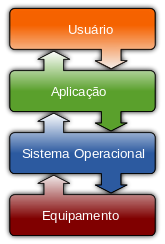
\includegraphics[width=0.4\textwidth]{img_so.png}
\centering
\caption{Representação da visão "top-down" e "bottom-up".}
\end{figure}

\chapter{Microsoft}
\label{chap.microsoft}

\section{História da Microsoft}

A Microsoft foi fundada no dia 4 de Abril de 1975, por Bill Gates e Paul Allen, na cidade de Albuquerque no estado "New Mexico".

A empresa Microsoft (incialmete chamada "Micro-Soft"), foi fundada com o a finalidade de produzir software para o primeiro microcomputador desenvolvido, o "Altair 8800". Para se dedicarem inteiramente á sua empresa, Paul Allen
demite-se do seu trabalho como programador em Boston, e Bill Gates decide sair da universidade de Harvard onde andava a estudar direito, isto deve-se ao facto de a empresa ser sediada em Albuquerque, pois foi lá é que foi desenvolvido o computador "Altair 8800" numa outra empresa chamada \acs{mits}.

\vspace{5mm}
\begin{figure}[h!]
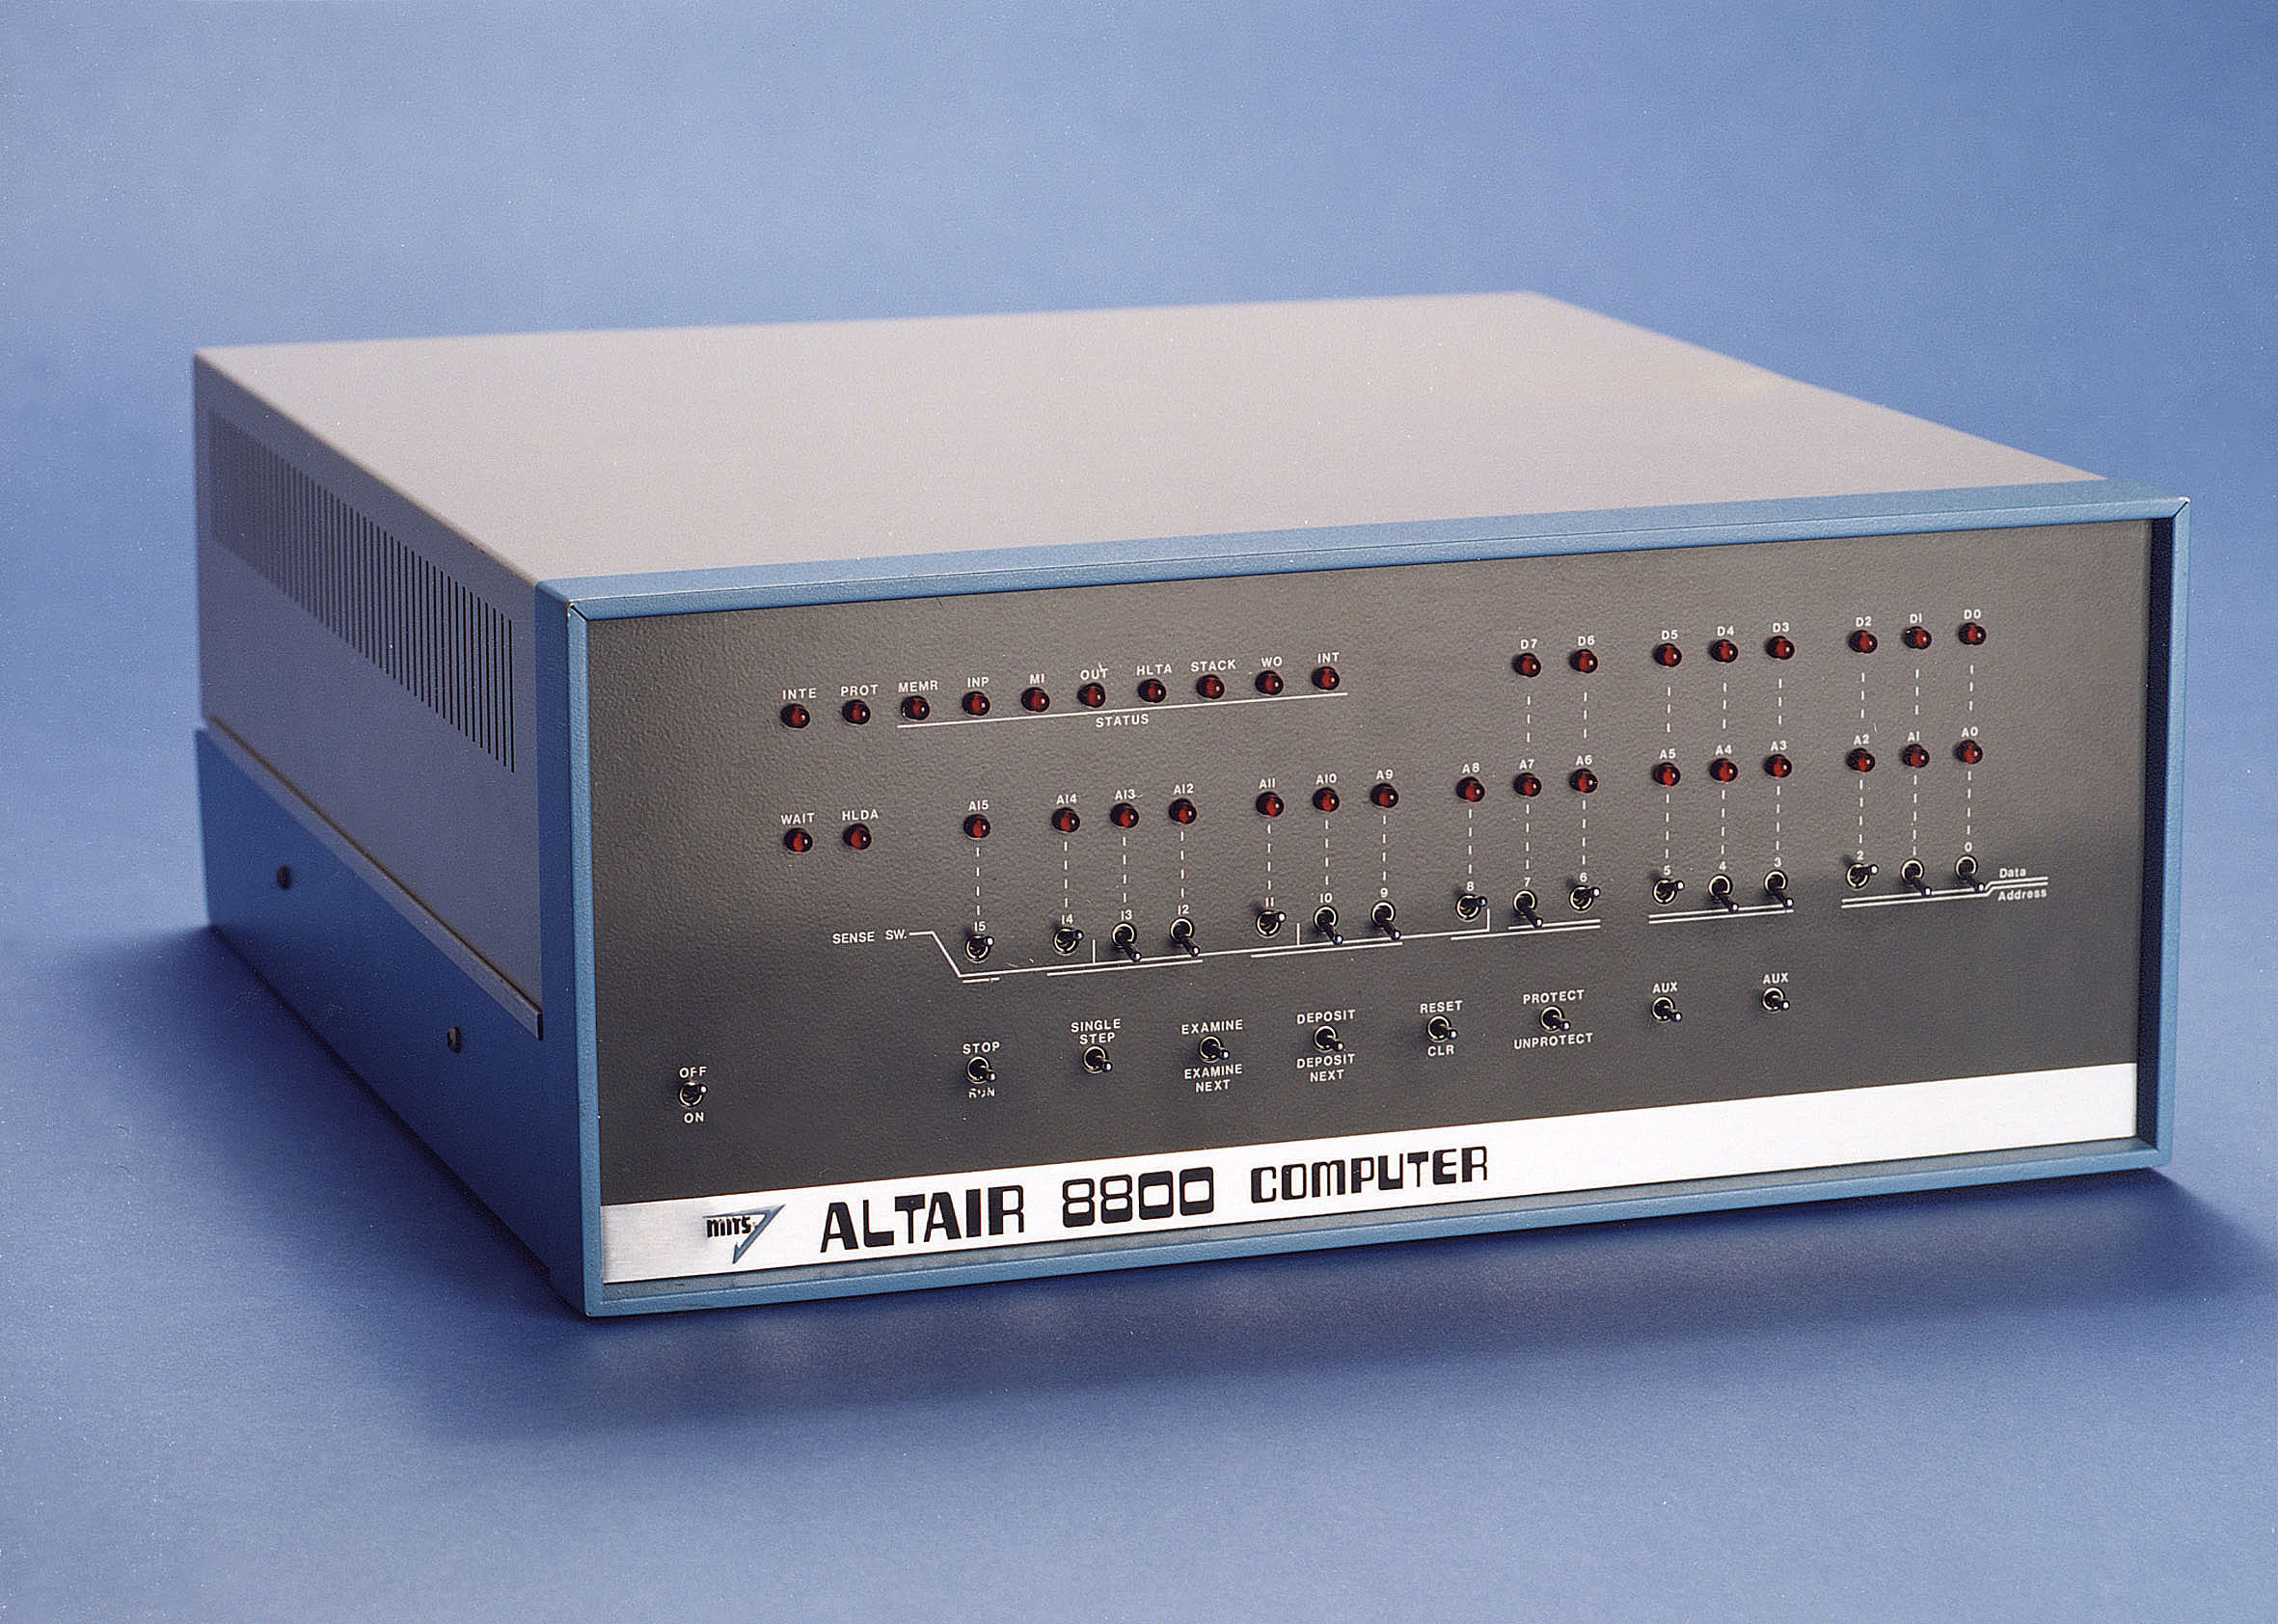
\includegraphics[width=0.5\textwidth]{altair-8800.jpg}
\centering
\caption{O Altair 8800}
\end{figure}
\vspace{5mm}

Gates e Allen propuseram criar um interpretador para o computador que tornasse possível a leitura da linguagem de programação "BASIC", de forma a tornar a máquina mais eficiente e capaz na realização de diversas tarefas.

Isto tudo foi possível com a ajuda de Monte Davidoff, um colega de de Bill Gates que também era especialista na linguagem de programação "BASIC".

Depois de terem criado o interpretador oito semanas antes da demonstração, chegou o "momento da verdade" e o interpretador funcionou corretamente sem qualquer tipo de falhas, ora isto fez com que a empresa \textbf{\ac{mits}} assinasse um contrato para começar a usar, e a divulgar o interpretador "Altair BASIC".

A partir deste momento, a Microsoft começou a marcar presença no mercado criando novas linguagens de programação, e a continuando a melhorar vários elementos da linguagem "BASIC".

Seguidamente, em 1980 a empresa \textbf{\ac{ibm}} pediu á Microsoft para desenvolver um software, neste caso um sistema operativo para o primeiro computador pessoal, o computador \acs{ibm}. Portanto, a Microsoft decidiu comprar um sistema operativo a uma empresa, e de seguida procederam á modificação do mesmo, nomeando-o \ac{ms-dos}.

\vspace{5mm}

Eventualmente, o sistema operativo acabou por ser lançado no ano de 1981, e grande parte das empresas que desenvolviam computadores pessoais decidiram adotar o \acs{ms-dos} como seu sistema operativo, consequentemente isto fez com que a Microsoft alcança-se mais de 100 milhões de vendas no ano 1990, adicionalmente destronou outros sistemas operativos que lideravam o mercado naquela altura tais como o "CP$\backslash$M" e o "IBM OS$\backslash$2".

\vspace{5mm}

\begin{figure}[h!]
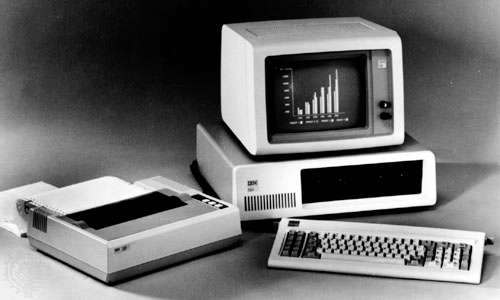
\includegraphics[width=0.5\textwidth]{IBM-Personal-Computer-machine-Microsoft-MS-DOS-operating-1981.jpg}
\centering
\caption{O computador IBM}
\end{figure}

\vspace{5mm}

Ainda no ano de 1990 a Windows lança uma interface gráfica  chamada "Windows" que basicamente consistia na  implementação de sistemas de janelas que tornavam o uso do computador mais intuitivo. A partir do ano de 1993 com o lançamento do Windows 3.0 e as suas versões posteriores, a Windows estava a vender 1 milhão de cópias por mês, e noventa porcento dos computadores de todo o mundo usavam o "Windows".

Em 1995 foi lançado o "Windows 95", que era basicamente uma fusão entre o "Windows" e o \acs{ms-dos}, e que naquela altura conseguiu ficar ao mesmo nível em termos de performance comparando com o computador da Apple, o MAC OS.

A partir desta altura, a Microsoft tornara-se uma das empresas mais lucrativas e poderosas da América com lucros superiores a 2 biliões de dólares, mesmo com a crise da "Grande Recessão" nos anos 2000 a empresa continuava a obter vencimentos extraordinários.

No entanto, a Microsoft focou-se tanto no desenvolvimento de sistemas operativos e outros softwares, que não se aperceberam da evolução dos sistemas redes e da Internet, e das potencialidades que estas ferramentas tinham. Então a Microsoft decidiu desenvolver um programa que se chama "Windows NT" cujo objetivo era conectar computadores diferentes entre si, isto tudo era possível tendo em conta um sistema de segurança. Inicialmente as vendas do programa ficaram aquém do desejado, mas em 1996 o "Windows NT" foi considerado o melhor programa para sistemas de redes no mercado, destronando o programa "Novell's Netware" da empresa Novell.

Depois disto, a Microsoft só voltou ao mercado de redes quando a empresa "Netscape Communications Corp." desenvolveu o navegador "Navigator", que simplificava o processo de navegar na Internet. A Microsoft quando soube disto, começou a trabalhar no desenvolvimento de um novo navegador o "Internet Explorer" que ainda existe nos dias de hoje. Para tornar este navegador, famoso e popular a Microsoft decidiu torná-lo grátis, consequentemente a empresa também tentou persuadir várias empresas de computadores e de serviços de Internet a usar este navegador exclusivamente.

No final de 1996, a Microsoft começou a vender o sistema operativo Windows com o "Internet Explorer" incluído.

\vspace{5mm}

\begin{figure}[h!]

\includegraphics[width=0.5\textwidth]{Internet-Explorer-logo.jpg}
\centering
\caption{O símbolo do Internet Explorer}
\end{figure}

\vspace{5mm}

\subsection{As funcionalidades e utilidades do Windows}
\label{sec.util}
Esta secção vai ser para falar das diferentes funcionalidades que o sistema operativo Windows oferece ao utilizador, lembrando que não vão ser faladas todas as funcionalidades, mas sim as mais importantes.

\begin{itemize}
    \item \textbf{Painel de Controlo:}
\end{itemize}

O painel de controlo consiste numa coleção de ferramentas que permite ao usuário configurar e gerir os recursos do seu computador. Neste painel é possível mudar as definições de uma impressora, definições de vídeo, áudio, rato e outros periféricos. Também é possível gerir contas de usuários, aplicações instaladas, conexões de rede, opções de gestão de energia e muitos outros.

\vspace{5mm}

\begin{figure}[h!]
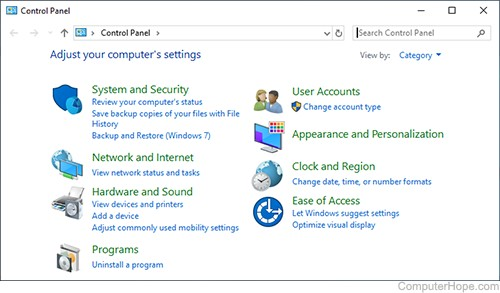
\includegraphics[width=0.7\textwidth]{cpanel-win10.jpg}
\centering
\caption{O painel de controlo}
\end{figure}

\vspace{5mm}

É possível aceder a este painel no menu inicial do Windows, em alternativa também é possível abrir este painel através da "Run box", basta usar o atalho \textbf{Win+R} escrever \textbf{control} e premir \underline{Enter}. Também para aceder ao painel através da Windows key, basta escrever "painel de controlo" e aceder.

\begin{itemize}
    \item \textbf{Cortana:}
\end{itemize}

A Cortana é um assistente virtual que foi introduzido no Windows 10 que é capaz de interpretar comandos de voz. Este assistente responde a perguntas feitas pelo o utilizador, navega na Internet, navega pelo sistemas de ficheiros do computador, é capaz de definir lembretes e fazer compras online e isto é apenas uma pequena parte das funções da Cortana.

Este assistente é muito semelhantes a outros que já estavam no mercado, tipo a \textbf{Siri} da Apple, a \textbf{Alexa} da Amazon, e o \textbf{Google Assistant} do Google.

\vspace{10mm}

Para aceder á Cortana basta usar o atalho \textbf{Win + S} e procurar por Cortana.

\begin{figure}[h!]
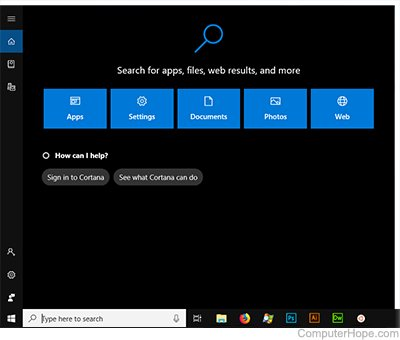
\includegraphics[width=0.7\textwidth]{cortana-win10.jpg}
\centering
\caption{A cortana}
\end{figure}

Para ativar os comandos de voz para a Cortana aceda este link: \url{https://www.computerhope.com/issues/ch001843.htm}

\vspace{35mm}

\begin{itemize}
    \item \textbf{Ambiente de Trabalho:}
\end{itemize}

O ambiente de trabalho é uma parte fundamental da interface gráfica do utilizador no Windows. Neste espaço dá para organizar, aplicações, documentos que aparecem com ícones no ambiente de trabalho. O ambiente de trabalho está sempre ativo no plano de fundo enquanto outras aplicações fazem as suas funções.

Isto é a primeira coisa que um utilizador vê quando liga o computador e inicia a sessão na sua conta do Windows. A partir daqui é possível aceder aos programas instalados pelo utilizador, clicando duas vezes no atalho da aplicação.

\begin{figure}[h!]
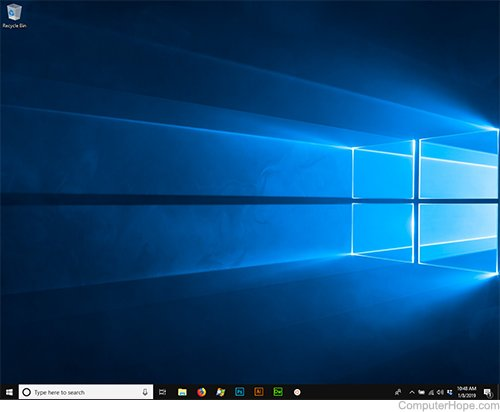
\includegraphics[width=0.5\textwidth]{desktop-win10.jpg}
\centering
\caption{O ambiente de trabalho}
\end{figure}

Para aceder ao ambiente de trabalho basta usar o atalho \textbf{Win + D}.

\begin{itemize}
    \item \textbf{Gestor de Dispositivos:}
\end{itemize}

O gestor de dispositivos faz uma lista de todo o hardware instalado no computador. Isto permite ao usuário atualizar os drivers (cuja função é aceitar requerimentos abstratos de software independente e transmiti-los ao hardware)  do hardware.

\begin{figure}[h!]
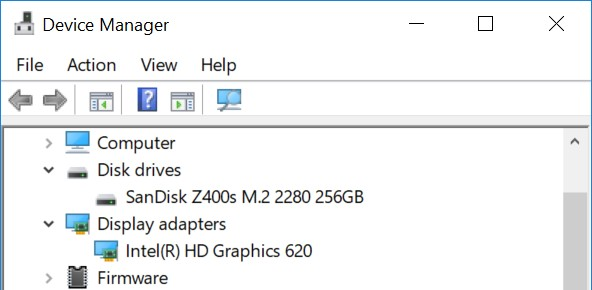
\includegraphics[width=0.7\textwidth]{device-manager.jpg}
\centering
\caption{O gestor de dispositivos}
\end{figure}

Para aceder ao gestor de dispositivos basta usar o atalho \textbf{Win + X} e depois selecionar "Gestor de dispositivos".

\begin{itemize}
    \item \textbf{Ferramenta de limpeza de disco:}
\end{itemize}

Esta ferramenta como o próprio nome indica, consiste na limpeza de itens desnecessários do disco. Usar esta ferramenta regularmente melhora a performance do computador, e aumenta o espaço para outros programas e documentos.

\begin{figure}[h!]
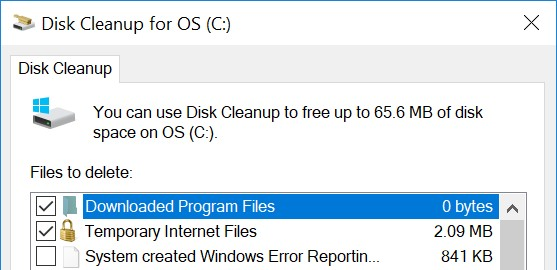
\includegraphics[width=0.7\textwidth]{disk-cleanup.jpg}
\centering
\caption{Limpeza do disco}
\end{figure}

Dá para aceder a esta ferramenta através do explorador de ficheiros.

\begin{enumerate}
    \item Use o atalho \textbf{Win + E} para aceder ao explorador de ficheiros;
    \item Na aba esquerda do explorador de ficheiros, encontre \textbf{Este PC} e abra essa aba;
    \item Seleciona a unidade de disco que queira limpar com o botão direito.
\end{enumerate}

\begin{itemize}
    \item \textbf{Visualizador de eventos:}
\end{itemize}

O visualizador de eventos é uma ferramenta de utilizador que mostra erros e eventos importantes que são executados no sistema. Isto ajuda a identificar vários erros que o computador possa ter.

\begin{figure}[h!]
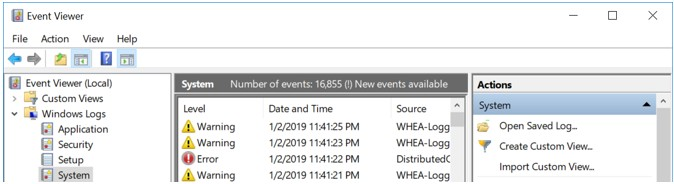
\includegraphics[width=1\textwidth]{event-viewer.jpg}
\centering
\caption{Visualizador de eventos}
\end{figure}

O visualizador de eventos pode ser acedido através do atalho \textbf{Win + X} e de seguida premindo \textbf{V}.

\begin{itemize}
    \item \textbf{Explorador de ficheiros:}
\end{itemize}

O explorador de ficheiros é uma ferramenta bastante intuitiva de usar, pois é das primeiras ferramentas com que o utilizador do sistema operativo se depara. Esta ferramenta permite navegar pelos conteúdos armazenados num \textbf{\acs{ssd}}, ou disco rígido, ou um disco externo. Também é possível procurar por ficheiros, eliminá-los, abri-los, ou mudar o nome dos mesmos.

\begin{figure}[h!]
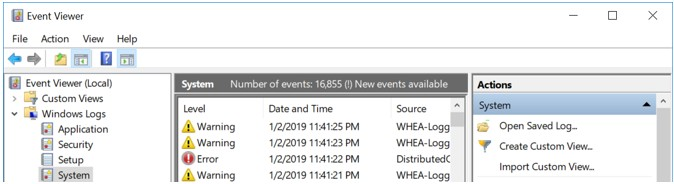
\includegraphics[width=1\textwidth]{event-viewer.jpg}
\centering
\caption{Explorador de ficheiros}
\end{figure}

Pode ser usado o atalho \textbf{Win + E} para aceder ao explorador de ficheiros. 
\begin{itemize}
    \item \textbf{Microsoft Paint:}
\end{itemize}

O Microsoft Paint é uma ferramenta quem tem vindo a ser implementada nos sistemas Windows desde 1985, esta é uma ferramenta que permite editar ou criar  imagens. Também permite ao utilizador desenhar e pintar imagens, e alterar o tamanho de fotografias.

\begin{figure}[h!]
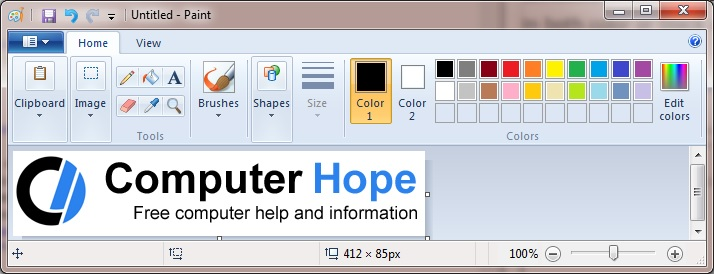
\includegraphics[width=1\textwidth]{paint.jpg}
\centering
\caption{Aplicação paint}
\end{figure}

Para aceder ao paint basta premir a tecla do Windows, escrever "mspaint" na barra de procura e clicar \underline{Enter}.

\begin{itemize}
    \item \textbf{Notepad:}
\end{itemize}

O Notepad é um editor de texto bastante simples. Esta ferramenta permite ao utilizador criar, ver e editar ficheiros de texto. A partir do Notepad, é possível criar ficheiros ".batch" ou escrever uma página web em \textbf{\acs{html}}.

\begin{figure}[h!]
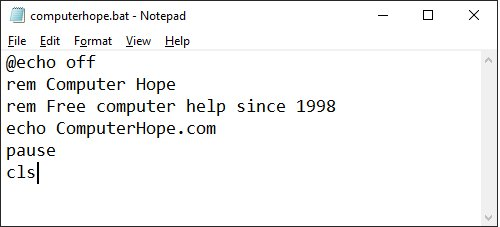
\includegraphics[width=1\textwidth]{notepad-computerhope.jpg}
\centering
\caption{O Notepad}
\end{figure}

Para aceder a aplicação Notepad basta usar o atalho \textbf{Win + R},  
escrever \textbf{notepad} e premir  \underline{Enter}.

\begin{itemize}
    \item \textbf{Editor de registo:}
\end{itemize}

O editor de registo permite ver o sistema de registo do Windows que é basicamente onde se armazena configurações de baixo nível para o sistema operativo. Esta ferramenta é bastante utilizada por técnicos de computadores, para reparar alguns erros de software instalado na máquina.

\begin{figure}[h!]
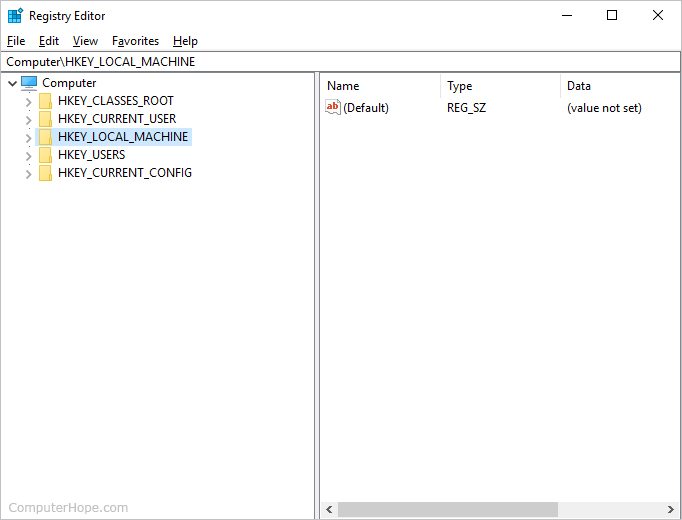
\includegraphics[width=1\textwidth]{registry-editor.jpg}
\centering
\caption{Editor de registo do Windows}
\end{figure}

O editor de registo do Windows pode ser acedido premindo a tecla do Windows e de seguida escrevendo \textbf{regedit} e premindo \underline{Enter}.

\begin{itemize}
    \item \textbf{Gestor de tarefas:}
\end{itemize}

O gestor de tarefas tem a funcionalidade de mostrar todos os processos que estão a ser executados no computador. Esta ferramenta também permite ver que processos requerem mais atenção, do processador, da placa gráfica e do disco, também permite encerrar processos que estão congelados ou que não respondem.

\vspace{35mm}

O gestor de tarefas pode ser invocado através do atalho \textbf{Crtl + Shift +Esc}.

\vspace{10mm}

\begin{figure}[h!]
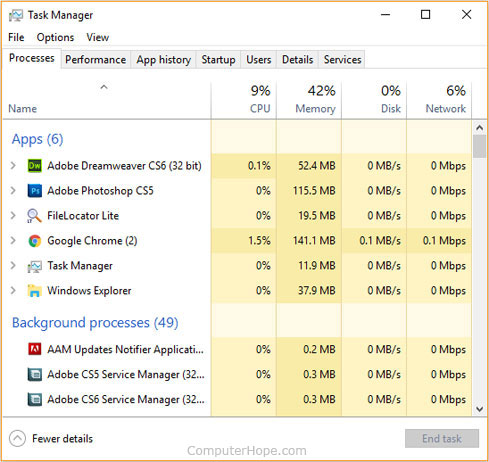
\includegraphics[width=1\textwidth]{taskmana10.jpg}
\centering
\caption{Gestor de tarefas do Windows}
\end{figure}

Para concluir este capítulo devo relembrar que estas ferramentas que foram indicadas aqui não são todas as ferramentas que o Windows oferece, existem muitas mais, mas se nós as metêssemos todas este documento iria ficar bastante extenso. 
Apenas indicámos aquelas mais importantes e essenciais do nosso ponto de vista.


\chapter{Linux}
\label{chap.linux}
O \textbf{Linux} é visto por grande parte das pessoas como um “simples” Sistema Operativo, no entanto o Linux é mais corretamente definido como um Kernel. Como referido antes, o Kernel é uma parte extremamente importante do Sistema Operativo, pois estabelece a ligação entre o processamento de dados e os programas.
No entanto este Kernel tem a particularidade de ser aberto, ao contrário do Kernel do Windows. Um Kernel aberto é um Kernel cujo \textbf{código-fonte} é aberto, pelo que pode ser editado por desenvolvedores ao redor do mundo. 
De uma maneira resumida, o código-fonte é um conjunto de comandos que após compilado ou interpretado dá origem a um software. Quando o código-fonte é aberto, como é o caso do Linux, é possível ver como é que este foi desenvolvido.

\section{História do Linux}

O Linux foi criado no ano de 1991 por \textit{Linus Torvalds}, um estudante de uma universidade na Finlândia. Para percebermos melhor a história do Linux teremos de falar primeiro dos sistemas operativos \textit{Minix} e \textit{Unix}.

\begin{figure}[h!]
    \centering
    \includegraphics[width=1\textwidth]{torvalds.jpeg}
    \caption{Linus Torvalds}
\end{figure}

\subsection{Minix}

O Linux não foi totalmente desenvolvido por Linus. Este foi desenvolvido a partir do \textbf{Minix}, que é um sistema Operacional desenvolvido por \textit{Andrew Stuart Tanenbaum}, um professor de computação, conhecido também por ser o autor dos livros “\textit{Redes de Computadores}”, “\textit{Sistemas Operacionais modernos}” e “\textit{Organização estruturada de computadores}” entre outros.

\begin{figure}[h!]
    \centering
    \includegraphics[width=1\textwidth]{tanenbaum.jpeg}
    \caption{Andrew S. Tanenbaum}
\end{figure}

\begin{figure}[h!]
    \centering
    \includegraphics[width=1\textwidth]{tanenbaumbook.jpeg}
    \caption{"Sistemas Operativos Modernos", Andrew S. Tanenbaum}
\end{figure}

O Minix foi lançado por Tanenbaum em 1987 com a principal finalidade de ser usado no ensino de computação, pois tratava-se de um sistema operacional simples e não exigia muitos recursos de \textit{hardware}.



\begin{figure}[h!]
    \centering
    \includegraphics[width=1\textwidth]{minix.jpeg}
    \caption{Logotipo do Minix}
\end{figure}

Devido ao facto de a finalidade de o Minix ser o ensino de computação, este foi disponibilizado gratuitamente, tal como o seu código-fonte completo, para que os estudantes pudessem criar os seus projetos baseados no Minix. Foi na qualidade de estudante que Linus Torvalds desenvolveu o Linux.

\subsection{Unix}

Tal como o Linux, o Minix não foi criado a partir do zero, este foi desenvolvido a partir do \textbf{Unix}, um sistema operacional com uma grande influência no mundo da computação.

\vspace{5mm}

O Unix surgiu em 1969, este era um projeto da \textit{Bell Labs}, um laboratório da AT\&T, mas apenas foi disponibilizado em meios académicos na década seguinte, o que levou ao seu desenvolvimento e surgimento de várias variações.

\begin{figure}[h!]
    \centering
    \includegraphics[width=1\textwidth]{at&t.jpeg}
    \caption{Logótipo da AT\&T}
\end{figure}
O Unix começou a ser desenvolvido em 1960 por um grupo de experientes programadores, entre eles Dennis Ritchie e Ken Thompson. Nessa altura o nome do projeto era Multics.

\begin{figure}[h!]
    \centering
    \includegraphics[width=1\textwidth]{unix1.jpeg}
    \caption{Ken Thompson(esquerda) e Dennis Ritchie(direita)}
\end{figure}
O Multics era um projeto bastante bom e ambicioso, mas foi inconcretizável, pois enfrentou diversos problemas, como a falta de recursos de hardware, pelo que Thompson decidiu criar o projeto Unics, um projeto mais realista e que pudesse ser realmente concretizado. Entretanto o nome do projeto foi alterado para Unix, como permanece até hoje. 

\vspace{5mm}

Ken Thompson e Dennis Ritchie são os nomes mais marcantes do grupo de desenvolvedores do Unix, pois em 1973 rescreveram todo o trabalho realizado no Unix até à data, utilizando linguagem C, uma linguagem desenvolvida por Dennis Ritchie, que após ser utilizada no Unix se tornou uma das principais linguagens a ser utilizada no desenvolvimento de Sistemas Operativos, fazendo assim de Dennis Ritchie um dos nomes mais reconhecidos desta área.

\begin{figure}
    \centering
    \includegraphics[width=1\textwidth]{c.jpeg}
    \caption{Logótipo da linguagem C}
\end{figure}

O Unix foi um dos projetos mais importantes na história da computação pois teve inúmeros sistemas operativos inspirados nele, que levaram a uma evolução muito mais rápida da área dos Sistemas Operativos.

\vspace{5mm}

\subsection{Linux}

Como já foi referido antes, Linus Torvalds era um estudante de ciências da computação na Universidade de Helsínquia, na Finlândia, onde começou a estudar em 1988 com 20 anos. Em 1990, cerca de 2 anos depois de entrar na universidade, Torvalds decidiu começar a desenvolver o seu Sistema Operativo, devido á sua insatisfação com o uso do Minix.
Em 1991 Torvalds já tinha um kernel funcional pelo que o divulgou na \textit{Usenet} (uma plataforma que permitia a troca de mensagens), com o intuito de obter opiniões e sugestões para que pudesse melhorar o seu trabalho.

\vspace{5mm}

Porém Linus Torvalds não fazia ideia do impacto que o Linux teria no mundo da tecnologia.

\begin{figure}[h!]
    \centering
    \includegraphics[width=1\textwidth]{linux.jpeg}
    \caption{Logótipo do Linux}
\end{figure}

No início Torvalds enfrentou duras criticas de Andrew Stuart Tanenbaum, criador do Minix. Tanenbaum achava o Linux “obsoleto” e afirmava que este tinha um design “monolítico”, ou seja, um design bastante básico e “sem vida”. Tanenbaum também não gostava do facto de o Linux estar feito para ser rodado apenas no processador \textbf{80386}, pois este era bastante caro, e seria eventualmente substituído por outro, o que não aconteceu.

\begin{figure}
    \centering
    \includegraphics[width=1\textwidth]{80386.jpeg}
    \caption{Exemplo de um processador 80386}
\end{figure}

Cada vez com mais colaboradores, Linus Torvalds seguiu com o seu trabalho, tornando o Linux disponível em outras plataformas.

\section{Nome}

Inicialmente, Linus designava o seu trabalho como \textit{Freax}, nome inspirado nas palavras “free” (grátis) e “freak” (monstruoso), e também um "x", para homenagear o Unix.
O nome Linux surgiu quando \textit{Ari Lemmke}, um colaborador de Linus, sugeriu colocar o projeto numa rede para que este se tornasse mais acessível. Este criou um servidor de FTP onde colocou uma pasta com o nome “linux”, pois não gostava do nome Freax. O nome Linux é a junção de Linus com Unix.

\section{GNU/Linux}
Como já foi referido, o Linux é apenas um Kernel e não um Sistema Operativo completo, pelo que necessita de ser executado com um conjunto de softwares para que possa ser utilizado. 

\vspace{5mm}

O \textbf{GNU}, sigla de “\textit{GNU’s not Unix}” (“Gnu não é Unix”) começou a ser desenvolvido em 1984 por \textit{Richard Stallman} que pretendia criar um sistema compatível com o Unix, mas sem utilizar o seu código.

\begin{figure}[h!]
    \centering
    \includegraphics[width=1\textwidth]{stallman.jpeg}
    \caption{Richard Stallman}
\end{figure}

Com o passar do tempo o GNU ia sendo desenvolvido, já tinha vários recursos, como compiladores e editores de texto, porem continuava a faltar uma parte importante do Sistema Operativo, o Kernel. Os desenvolvedores do GNU trabalhavam na criação de um Kernel de nome \textit{Hurd}, porem, devido á demora que a criação deste kernel estava a levar, muitos utilizadores começaram a usar o GNU com o kernel Linux.

\vspace{5mm}

O Linux que conhecemos hoje em dia continua a funcionar com software GNU, pelo que algumas pessoas ligadas ao desenvolvimento de Sistemas Operativos defendem que se deveria chamar ao conjunto do Linux com GNU "\textbf{GNU/Linux}", porém grande parte das pessoas continua a chamar ao conjunto "Linux", pois foi criado esse habito.


\begin{figure}[h!]
    \centering
    \includegraphics[width=1\textwidth]{gnu.jpeg}
    \caption{Logótipo do GNU (esquerda) acompanhado do logótipo do Linux (direita)}
    \label{fig:my_label}
\end{figure}


\section{Distribuições Linux}

Devido ao facto de o Linux ser um kernel disponível gratuitamente, qualquer pessoa ou entidade pode criar o seu sistema operativo customizado, juntando o Linux a um conjunto de softwares, podendo assim obter um sistema operativo com as funcionalidades desejadas. Cada sistema operativo destes é designado “\textbf{Distribuição Linux}” ou “\textbf{Distribuição GNU/Linux}”.

\vspace{5mm}

Existem inúmeras distribuições de Linux com os mais diversos fins, mas as distribuições para o uso doméstico são as mais populares.

\begin{figure}[h!]
    \centering
    \includegraphics[width=1\textwidth]{distributions.jpeg}
    \caption{Vários exemplos de distribuições Linux}
\end{figure}

Atualmente a distribuição mais utilizada é o \textbf{Ubuntu}, da empresa \textit{Canonical}. O seu lançamento ocorreu em outubro de 2004. Este sofre atualizações de meio em meio ano (Outubro e Abril) para que se possa manter sempre ao nível de exigência dos seus utilizadores.
Até 2017 existia também o Ubuntu para telemóveis e tablets, o \textit{Ubuntu Touch}, porem após não ter tanto sucesso, deixou de ser comercializado. 

\begin{figure}[h!]
    \centering
    \includegraphics[width=1\textwidth]{ubuntu.jpeg}
    \caption{Computador com Ubuntu}
\end{figure}

Outro Sistema Operativo bastante utilizado, baseado no kernel Linux é o \textbf{Android}, utilizado em principalmente em tablets e telemóveis, mas também em carros, smartwatches, entre outros. O Android é o Sistema Operativo móvel mais utilizado no mundo. As suas vendas superam as vendas de dispositivos Windows, iOS e macOS todas juntas.
O Android foi desenvolvido por uma equipa designada \textit{Open Handset Alliance}, sendo um dos principais colaboradores o \textit{Google}.

\begin{figure}
    \centering
    \includegraphics[width=1\textwidth]{android.jpeg}
    \caption{Logótipo do Android}
\end{figure}

Existem também outras distribuições bastante usadas, como por exemplo: 

\begin{itemize}
    \item Debian
    \item Fedora 
    \item Arch Linux
    \item Linux Mint
    \item CentOS
    \item Slackware
\end{itemize}

\section{Licença do Linux}

Uma \textit{licença} é um documento que indica ao utilizador aquilo que pode ser, ou não, feito com um software. A licença utilizada pelo Linux é a \textbf{GPL} (\textit{GNU General Public License}). Inicialmente a licença usada tinha sido criada por Linus Torvalds e incluía restrições para o uso comercial. A GPL começou a ser usada pelo Linux em 1992.

\vspace{5mm}

A GPL, criada pela fundação Free Software Foundation, criada por Richard Stallman, desenvolvedor do GNU. A GPL foca-se nos seguintes tópicos:

\begin{itemize}
    \item Liberdade para executar o programa, com qualquer finalidade (liberdade 0);
    \item Liberdade de estudar a forma como o programa funciona e adapta-lo ás suas necessidades (liberdade 1);
    \item Liberdade de distribuir cópias de forma a ajudar outros indivíduos (liberdade 2);
    \item Liberdade de melhorar e aperfeiçoar o software, de modo a que todos sejam beneficiados (liberdade 3).
\end{itemize}

Nos tópicos liberdade 1 e liberdade 3, o acesso ao código fonte é necessário, caso contrário um software não poderá usar a GPL.

\chapter{MacOS}
\label{chap.macos}

O \textbf{macOS} é um sistema operativo desenvolvido pela \textit{Apple} desde 2001 e destina-se apenas aos computadores \textit{Mac} da apple. Tal como no GNU/Linux, o kernel deste sistema operativo baseia-se no Unix e é designado \textbf{XNU} (X’s Not Unix), e é combinado com uma interface gráfica \textit{GUI} (Graphical User Interface). Na primeira versão do macOS foram utilizados o kernel XNU e uma GUI designada \textit{Aqua}.

\begin{figure}[h!]
    \centering
    \includegraphics[width=1\textwidth]{apple.jpeg}
    \caption{Logotipo da Apple}
\end{figure}

O macOS é um sistema operativo conhecido principalmente pela qualidade dos seus gráficos. Este utiliza bordas arredondadas, uma grande variedade de cores translucidas e outros pormenores bastante apelativos, pelo que na sua criação sofreu várias criticas como “parece um brinquedo” e a Apple foi criticada por alegada falta de profissionalismo.

\begin{figure}[h!]
    \centering
    \includegraphics[width=1\textwidth]{mac.jpeg}
    \caption{Portátil Mac com o sistema operativo Mac OS}
\end{figure}


\section{História do MacOS}

A historia do macOS começou a ser escrita na \textbf{NeXT}, uma empresa fundada por \textit{Steve Jobs} quando saiu da Apple em 1985. Em 1989 foI lançado o \textbf{Unix-like NeXTSTEP}, um Sistema Operativo baseado no Kernel \textit{Mach}, previamente desenvolvido na \textit{Carnegie Mellon University} a partir do \textbf{BSD} (\textit{Berkeley Software Distribution}), um derivado do Unix.  A interface gráfica foi feita através de uma GUI toolkit usando a linguagem de programação \textbf{Objective-C}.

\begin{figure}[h!]
    \centering
    \includegraphics[width=1\textwidth]{stevejobs.jpeg}
    \caption{Steve Jobs}
\end{figure}

No incio dos anos 90, a Apple tentava desenvolver um sistema operativo para os seus novos Macs, porem devido a vários insucessos viram-se obrigados a comprar o NeXTSTEP em 1996, processo que fez Steve Jobs voltar á Apple. Após a compra do NeXTSTEP, vários programadores trabalharam para adequar este sistema operativo ao pretendido pela Apple. Este projeto foi inicialmente designado “Rhapsody” tendo sido posteriormente alterado para \textbf{MacOS}

\section{Versões do macOS}

Foram lançadas ao todo 17 versões do macOS, inicialmente, a todas elas era atribuído o nome de um felino, porem devido á falta de nomes, as diferentes versões começaram a ter nomes de lugares icónicos do estado da Califórnia, onde fica sediada a Apple.

Segue-se uma lista das diferentes versões:

\begin{itemize}
    \item MacOS X v10.0 “Cheetah”
    \item MacOS X v10.1 “Puma”
    \item MacOS X v10.2 “Jaguar”
    \item MacOS X v10.3 “Panther”
    \item MacOS X v10.4 “Tiger”
    \item MacOS X v10.5 “Leopard”
    \item MacOS X v10.6 “Snow Leopard”
    \item MacOS X v10.7 “Lion”
    \item OS X v10.8  ”Mountain Lion”
    \item OS X v10.9 ”Mavericks”
    \item OS X v10.10 “Yosemite”
    \item OS X v10.11 “El Capitan”
    \item MacOS  v10.12 “Sierra”
    \item MacOS v10.13”High Sierra”
    \item MacOS v10.14 “Mojave”
    \item MacOS v10.15 “Catalina”
    \item MacOS v10.16 ”Big Sur”
\end{itemize}


\chapter{Análise}
\label{chap.analise}
Ao longo deste trabalho pudemos ler sobre os mais influentes Sistemas Operativos até á atualidade. 

\vspace{5mm}

Sendo o Windows um Sistema Operativo bastante fácil de ser utilizado, razão pela qual é o Sistema Operativo para computadores mais vendido em todo o mundo. 
\vspace{5mm}

Vimos também que o Linux é apenas um kernel, não sendo por isso um Sistema Operativo na sua totalidade. Mas pode ser executado com outros softwares de modo a formar um Sistema Operativo por inteiro, pelo que existe uma enorme diversidade de distribuições Linux, com os mais diversos fins.

\vspace{5mm}

Vimos ainda que o MacOS, Sistema Operativo dos computadores Mac da Apple, também deriva do Unix, tal como o Linux. Este é um Sistema Operativo mais focado na qualidade dos gráficos e animações.


\chapter{Conclusões}
\label{chap.conclusao}

Para concluir, pudemos observar ao longo deste trabalho que existe uma enorme variedade de Sistemas Operativos, cada um com a sua particularidade. Apesar de nós só termos abordado os 3 mais conhecidos, existem ainda muitos outros Sistemas Operativos, que podem ser utilizados, tanto para uso doméstico, como para fins de trabalho.
Pudemos também ler a história destes 3 Sistemas Operativos, que são bastante inspiradoras para qualquer estudante da área da informática.

\chapter*{Contribuições dos autores}
O trabalho foi realizado por partes, tendo sido cada uma delas atribuída a um dos alunos. Após várias sugestões de ambas as partes o tema para a realização do trabalho foi escolhido. O aluno \acs{bg} realizou o resumo, introdução e desenvolveu o tema Microsoft, enquanto aluno \acs{ja} desenvolveu os temas Linux e MacOS, e escreveu a analise e conclusões retiradas da realização do trabalho.
Podemos então afirmar que cada um dos alunos \acs{bg} e \acs{ja} realizou 50\% do trabalho.

\begin{thebibliography}{}
\bibitem{brittanicawebsite}
\url{https://www.britannica.com/topic/Microsoft-Corporation}

\bibitem{wikipedia}
\url{https://en.wikipedia.org/wiki/History_of_Microsoft}

\bibitem{historywebsite}
\url{https://www.history.com/this-day-in-history/microsoft-founded}

\bibitem{computerhope}
\url{https://www.computerhope.com/issues/ch001967.htm#controlpanel}

\bibitem{wikipedia}
\url{https://pt.wikipedia.org/wiki/Linux}

\bibitem{sitesapo}
\url{https://pplware.sapo.pt/category/linux/}

\bibitem{wikipedia}
\url{https://pt.wikipedia.org/wiki/Unix}

\bibitem{universidadedominho}
\url{http://piano.dsi.uminho.pt/museuv/UNIX.html}

\bibitem{wikipedia}
\url{https://pt.wikipedia.org/wiki/MacOS}

\bibitem{wikipedia}
\url{https://pt.wikipedia.org/wiki/Ubuntu}

\bibitem{crazyprogrammer}
\url{https://www.thecrazyprogrammer.com/2019/12/advantages-and-disadvantages-of-operating-system.html}
\end{thebibliography}

%%%%%%%%%%%%%%%%%%%%%%%%%%%%%%%%%
\chapter*{Acrónimos}
\begin{acronym}
\acro{ua}[UA]{Universidade de Aveiro}
\acro{miect}[MIECT]{Mestrado Integrado em Engenharia de Computadores e Telemática}
\acro{lei}[LEI]{Licenciatura em Engenharia Informática}
\acro{glisc}[GLISC]{Grey Literature International Steering Committee}
\acro{mits}[MITS]{Micro Instrumentation and Telemetry Systems}
\acro{ibm}[IBM]{International Business Machines Corporation}
\acro{ms-dos}[MS-DOS]{Microsoft Disk Operating System}
\acro{ssd}[SSD]{Solid State Drive}
\acro{html}[HTML]{Hyper Text Markup Language}
\acro{rom}[ROM]{Read-Only Memory}
\acro{bios}[BIOS]{Basic Input/Output System}
\acro{bg}[BG]{Bruno Gomes}
\acro{ja}[JA]{João Artur}
\end{acronym}


%%%%%%%%%%%%%%%%%%%%%%%%%%%%%%%%%
\printbibliography

\end{document}
